\section{Normal Distribution/ Gaussian Distribution (${N}(\mu, \sigma^2)$)}


\begin{table}[H]
    \hfill
    \begin{minipage}{0.45\linewidth}
        \begin{figure}[H]
            \centering
            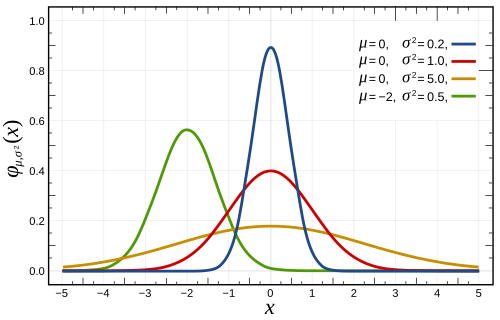
\includegraphics[
                width=\linewidth,
                height=5cm,
                keepaspectratio,
            ]{images/distributions/Normal_Distribution_PDF.svg.png}
            \caption{Normal Distribution: PDF \cite{wiki/Normal_distribution}}
        \end{figure}
    \end{minipage}
    \hfill
    \begin{minipage}{0.45\linewidth}
        \begin{figure}[H]
            \centering
            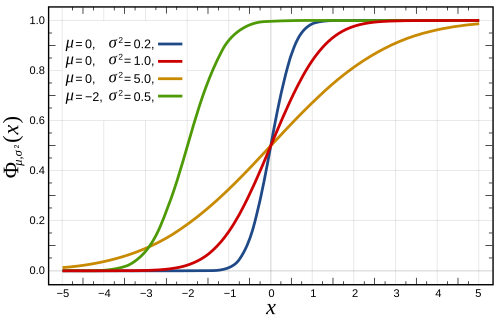
\includegraphics[
                width=\linewidth,
                height=5cm,
                keepaspectratio,
            ]{images/distributions/Normal_Distribution_CDF.svg.png}
            \caption{Normal Distribution: CDF \cite{wiki/Normal_distribution}}
        \end{figure}
    \end{minipage}
    \hfill
\end{table}

\begin{enumerate}
    \item Denoted by: $\mathcal{N}(\mu, \sigma^2)$
\end{enumerate}


\subsection{PDF ($f_{\mu, \sigma}(x)$ or $f(x|\mu, \sigma)$)}

\begin{enumerate}
    \item[]  $
        f_{\mu, \sigma}(x)
        = \dfrac{1}{\sigma\sqrt{2\pi}} \exp\dParenBrac{-\dfrac{(x-\mu)^2}{2\sigma^2}}
    $ 
    \hfill \cite{statistics/book/Statistics-for-Data-Scientists/Maurits-Kaptein}
    \begin{enumerate}
        \item[] $\mu \in \mathbb{R}$: indicates the mean value of the population of the variable of interest
        \hfill \cite{statistics/book/Statistics-for-Data-Scientists/Maurits-Kaptein}

        \item[] $\sigma$: indicates the standard deviation ($\sigma^2 > 0$)
        \hfill \cite{statistics/book/Statistics-for-Data-Scientists/Maurits-Kaptein}
    \end{enumerate}

    \item[] $f_{\mu, \sigma}(x) = \dfrac{1}{\sigma}\phi\dParenBrac{\dfrac{x-\mu}{\sigma}}$
    \hfill \cite{statistics/book/Statistics-for-Data-Scientists/Maurits-Kaptein}

    \item it can be used to approximate other PDFs when the sample size or the size of the data is getting large.
    \hfill \cite{statistics/book/Statistics-for-Data-Scientists/Maurits-Kaptein}

    \item This has the advantage that important features of the normal density function can be transferred to other densities when the approximation is quite close. 
    \hfill \cite{statistics/book/Statistics-for-Data-Scientists/Maurits-Kaptein}

    \item The shape of the normal PDF is equal to the famous “bell-shape” curve 
    \hfill \cite{statistics/book/Statistics-for-Data-Scientists/Maurits-Kaptein}

    \item areas under the curve:
    \begin{enumerate}
        \item $99.73\%$ of all the population values fall within the interval $[\mu - 3\sigma, \mu + 3\sigma]$
        \hfill \cite{statistics/book/Statistics-for-Data-Scientists/Maurits-Kaptein}
    
        \item $95.45\%$ of all the population values fall within the interval $[\mu - 2\sigma, \mu + 2\sigma]$ or 
        \hfill \cite{statistics/book/Statistics-for-Data-Scientists/Maurits-Kaptein}
        \\
        $
            \dint_{\mu - 2\sigma}^{\mu + 2\sigma}
            \phi\dParenBrac{\dfrac{x-\mu}{\sigma}} dx
            = 
            \dint_{-2}^{2}
            \phi(x) dx
            =
            0.9545
        $
        \hfill \cite{statistics/book/Statistics-for-Data-Scientists/Maurits-Kaptein}

        \item $95\%$ of the values fall within $[\mu - 1.96\sigma, \mu + 1.96\sigma]$
        \hfill \cite{statistics/book/Statistics-for-Data-Scientists/Maurits-Kaptein}
    \end{enumerate}

    \item  describes both positive and negative values
    \hfill \cite{statistics/book/Statistics-for-Data-Scientists/Maurits-Kaptein}

    \item a random measurement error that could be described by a normal PDF is more likely to be closer to zero than to be further away from zero (due to the bell shape of the density). 
    \hfill \cite{statistics/book/Statistics-for-Data-Scientists/Maurits-Kaptein}
\end{enumerate}




\subsection{Summary}

\begin{enumerate}

    \item 
    \textbf{Notation}:
    $
        {\displaystyle {\mathcal {N}}(\mu ,\sigma ^{2})}
    $
    \hfill \cite{wiki/Normal_distribution} 

    \item 
    \textbf{Parameters}:
    \begin{enumerate}
        \item ${\displaystyle \mu \in \mathbb {R} }$ = mean (location)
        \hfill \cite{wiki/Normal_distribution}

        \item ${\displaystyle \sigma ^{2}\in \mathbb {R} _{>0}}$ = variance (squared scale)
        \hfill \cite{wiki/Normal_distribution}
    \end{enumerate}

    \item 
    \textbf{Support/ Rand Var}: 
    $x \in \mathbb{R}$ 
    \hfill \cite{wiki/Normal_distribution}

    \item 
    \textbf{PDF}: 
    $ {\displaystyle {\dfrac {1}{\sqrt {2\pi \sigma ^{2}}}}e^{-{\dfrac {(x-\mu )^{2}}{2\sigma ^{2}}}}} $ 
    \hfill\cite{wiki/Normal_distribution}

    \item 
    \textbf{CDF}: 
    $ {\displaystyle \Phi \left({\dfrac {x-\mu }{\sigma }}\right)={\dfrac {1}{2}}\left[1+\operatorname {erf} \left({\dfrac {x-\mu }{\sigma {\sqrt {2}}}}\right)\right]} $ 
    \hfill\cite{wiki/Normal_distribution}

    \item 
    \textbf{Quantile}:
    $ {\displaystyle \mu +\sigma {\sqrt {2}}\operatorname {erf} ^{-1}(2p-1)} $ 
    \hfill\cite{wiki/Normal_distribution}

    \item 
    \textbf{Mean}:
    $ {\displaystyle \mu } $ 
    \hfill\cite{wiki/Normal_distribution}

    \item 
    \textbf{Median}:
    $ {\displaystyle \mu } $ 
    \hfill\cite{wiki/Normal_distribution}

    \item 
    \textbf{Mode}:
    $ {\displaystyle \mu } $ 
    \hfill\cite{wiki/Normal_distribution}

    \item 
    \textbf{Variance}:
    $ {\displaystyle \sigma ^{2}} $
    \hfill\cite{wiki/Normal_distribution}

    \item 
    \textbf{Median absolute deviation (MAD)}:
    $ {\displaystyle \sigma {\sqrt {2}}\,\operatorname {erf} ^{-1}(1/2)} $
    \hfill\cite{wiki/Normal_distribution}

    \item 
    \textbf{Average absolute deviation (AAD)}:
    $ {\textstyle \sigma {\sqrt {2/\pi }}} $
    \hfill\cite{wiki/Normal_distribution}

    \item 
    \textbf{Skewness}: $0$
    \hfill\cite{wiki/Normal_distribution}

    \item 
    \textbf{Excess kurtosis}: $0$
    \hfill\cite{wiki/Normal_distribution}

    \item 
    \textbf{Entropy}: $ {\textstyle {\tfrac {1}{2}}\log(2\pi e\sigma ^{2})} $
    \hfill\cite{wiki/Normal_distribution}

    \item 
    \textbf{Moment-generating function (MGF)}: $ {\displaystyle \exp(\mu t+\sigma ^{2}t^{2}/2)} $ 
    \hfill\cite{wiki/Normal_distribution}

    \item 
    \textbf{Characteristic function (CF)}: $ {\displaystyle \exp(i\mu t-\sigma ^{2}t^{2}/2)} $ 
    \hfill\cite{wiki/Normal_distribution}

    \item 
    \textbf{Fisher information}:
    \begin{enumerate}
        \item ${\displaystyle {\mathcal {I}}(\mu ,\sigma )={\begin{pmatrix}1/\sigma ^{2}&0\\0&2/\sigma ^{2}\end{pmatrix}}}$

        \item ${\displaystyle {\mathcal {I}}(\mu ,\sigma ^{2})={\begin{pmatrix}1/\sigma ^{2}&0\\0&1/(2\sigma ^{4})\end{pmatrix}}}$
    \end{enumerate}
    \hfill\cite{wiki/Normal_distribution}
    
    \item 
    \textbf{Kullback–Leibler divergence}:
    ${\displaystyle D_{KL} = {1 \over 2}\left\{\left({\dfrac {\sigma _{0}}{\sigma _{1}}}\right)^{2}+{\dfrac {(\mu _{1}-\mu _{0})^{2}}{\sigma _{1}^{2}}}-1+\ln {\sigma _{1}^{2} \over \sigma _{0}^{2}}\right\}}$
    \hfill\cite{wiki/Normal_distribution}

    \item 
    \textbf{Expected shortfall}:
    ${\displaystyle \mu +\sigma {\dfrac {{\dfrac {1}{\sqrt {2\pi }}}e^{\dfrac {-\left(q_{p}\left({\dfrac {X-\mu }{\sigma }}\right)\right)^{2}}{2}}}{1-p}}}$
    \hfill\cite{wiki/Normal_distribution}

\end{enumerate}

